\section{Durchführung als Projekt}
\subsection{Ziele}
\steffen
Ziel der Unterrichtsreihe ist es, die Schüler den mathematischen Modellierungskreislauf herleiten und durchführen zu lassen. Als Modellierungsobjekt dient dabei die Modellierung von Epidemien und Pandemien. 


\begin{landscape}
\subsection{Reihenplanung}
\noindent
\begin{longtable}{|C{0.05\textwidth}|L{0.2\textwidth}|L{0.3\textwidth}|L{0.25\textwidth}|L{0.3\textwidth}|L{0.25\textwidth}|L{0.1\textwidth}|}
\hline
Std&Inhalte&Grobziele \& Kompetenzen&Wdh \& Festigung&didakt. \& method. Auswahl&Medien&Sonstiges\\
\hline\hline
\endhead
\hline
\endfoot
1\&{}2 &\emph{SIHDR}&\begin{itemize}
	\item Schüler durchlaufen den Modellierungskreislauf zwei mal
	\item K2
	\item K3
\end{itemize}&--&\begin{itemize}
	\item Modell von \emph{SID} zu \emph{SIHDR}
	\item TPS zur Modellbildung
	\item Zwischenergebnisse werden in der Klasse besprochen
	\item Durch Aufgabenstellung wenig Varianz in Modellierung
\end{itemize}&\begin{itemize}
	\item Ta\-bel\-len\-kal\-ku\-la\-tion
\end{itemize}&--\\\hline
3\&{}4&\begin{itemize}
	\item Mo\-del\-lier\-ungs\-kreis\-lauf
	\item \emph{SIHFDR}
\end{itemize}&b&c&d&e&f\\\hline
5\&{}6&\begin{itemize}
	\item Maß\-nahmen gegen Ausbreitung
	\item Schwächen des Modells
	\item Erwei\-terung auf mehrere Nationen
\end{itemize}&\begin{itemize}
	\item K2
	\item K3
\end{itemize}&Model der Vorstunde&d&e&f\\
\end{longtable}
\end{landscape}
\subsection{Projektstunde 1 \& 2}\ellen
\subsubsection{Bemerkungen zur Lerngruppe}
\subsubsection{Methodische Überlegungen}
%\subsubsection{Verlaufsskizze}
\begin{landscape}
\subsubsection{Verlaufsskizze}
\noindent
\begin{tabular}{|C{0.3\textwidth}|L{0.8\textwidth}|L{0.4\textwidth}|}
\hline
Phase & Arbeitsauftrag & Sozialform\\
\hline\hline
Begrüßung & keine & Lehrervortrag\\
\hline
Einstieg & Lesen der Informationen über Ebola & Einzelarbeit\\
\hline
1. Erarbeitungsphase (a) & Modell entwickeln zur Simulation einer Ebola Epidemie & Einzelarbeit\\
\hline
1. Erarbeitungsphase (b) & Modell mit dem Nachbarn vergleichen, ein gemeinsames Modell erarbeiten & Partnerarbeit\\
\hline
1. Erarbeitungsphase (c) & Das gemeinsame Modell mit Hilfe von Tabellenkalkulationsprogramm simulieren & Partnerarbeit\\
\hline
1. Reflexionsphase & Modelle der SuS werden vorgestellt und Stärken und Schwächen der Modelle besprochen & Schülervorträge + Diskussion\\
\hline
2. Erarbeitungsphase & Mit neuen Informationen und den Überlegungen aus der Diskussion wird das Modell verbessert und wieder eine Simulation durchgeführt & Partnerarbeit\\
\hline
\end{tabular}
\end{landscape}
\subsubsection{Materialien}
\noindent\frame{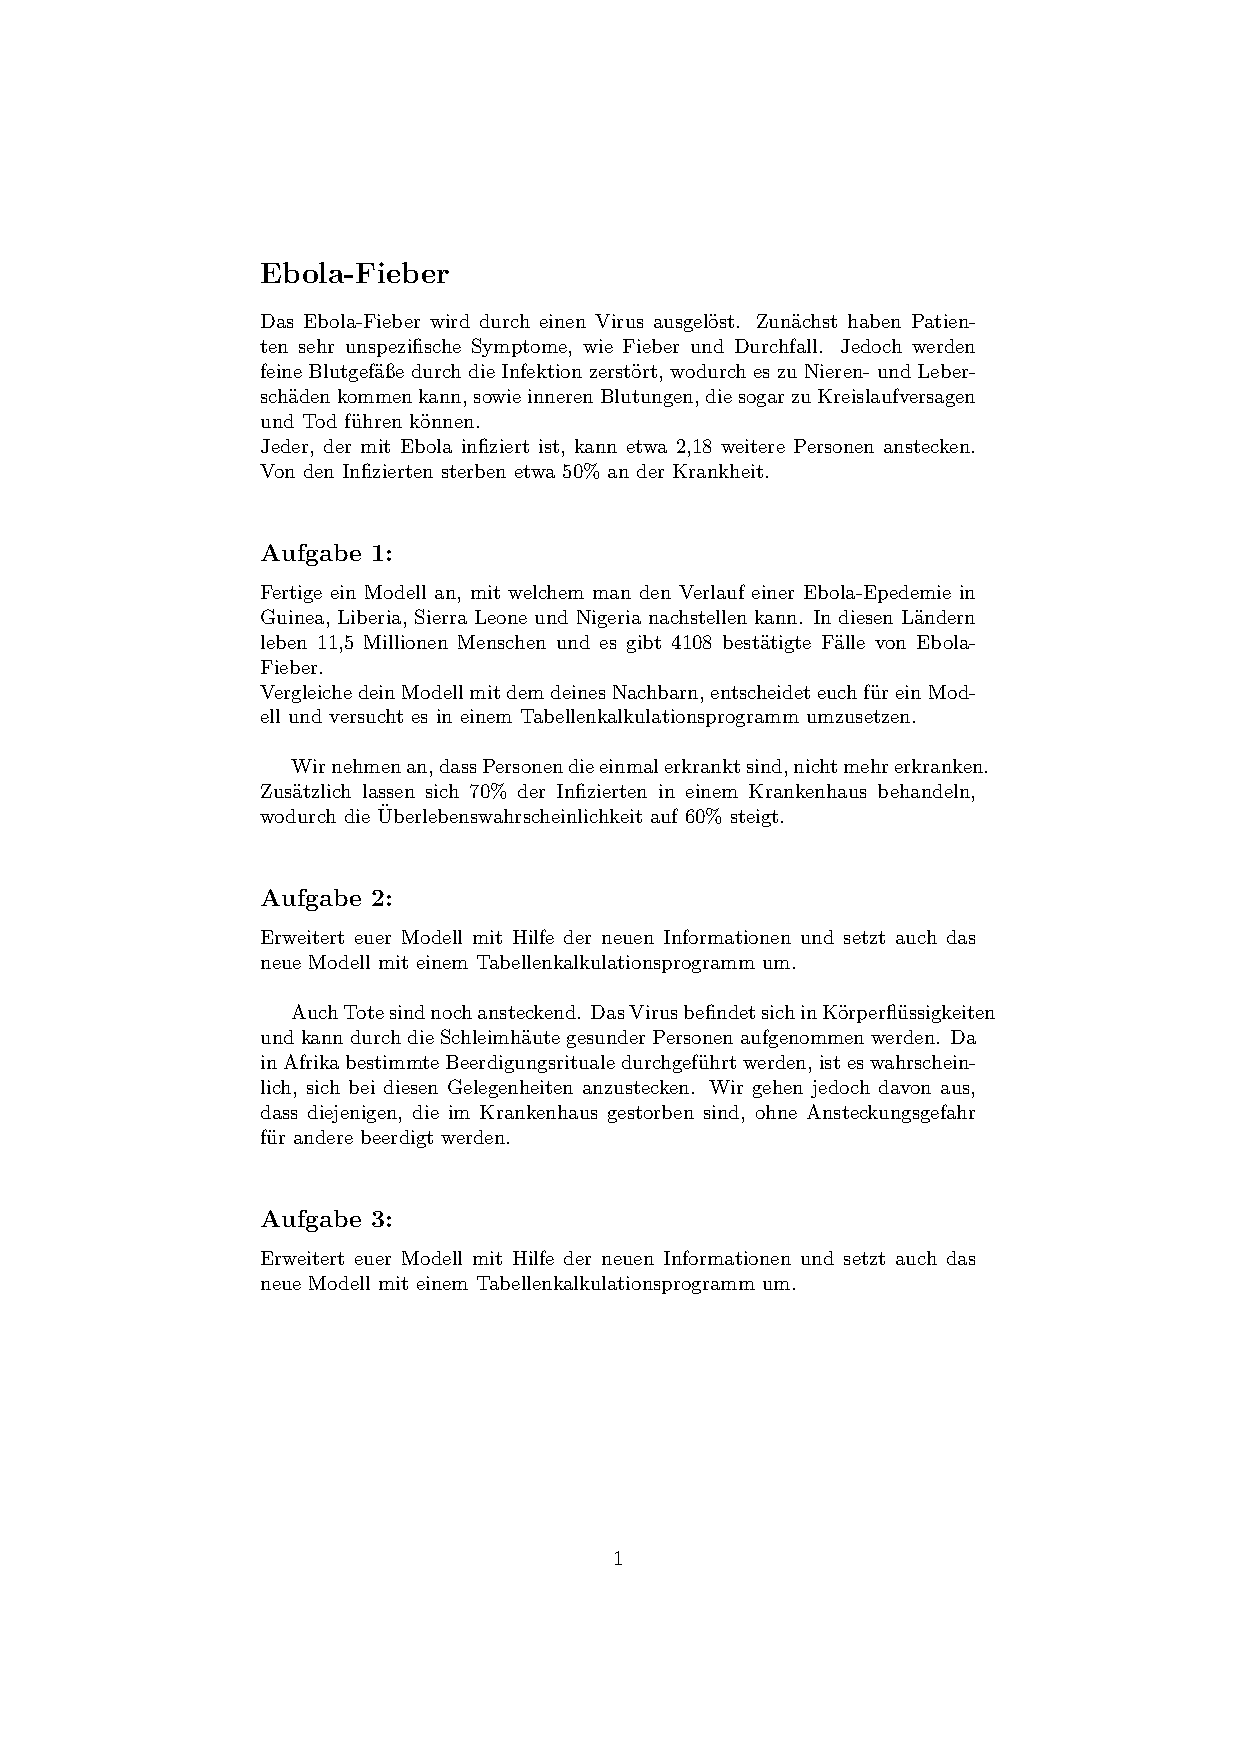
\includegraphics[width=\textwidth]{projekt/Arbeitsblatt_1}}
\subsubsection{Erwartungshorizont}
\subsubsection{Reflexion der Stunde}
\newpage
\subsection{Projektstunde 3 \& 4}\ellen
\subsubsection{Bemerkungen zur Lerngruppe}
\subsubsection{Methodische Überlegungen}
\subsubsection{Verlaufsskizze}
\subsubsection{Materialien}
\subsubsection{Erwartungshorizont}
\subsubsection{Reflexion der Stunde}
\newpage
\subsection{Projektstunde 5 \& 6}\steffen
\subsubsection{Bemerkungen zur Lerngruppe}
\subsubsection{Methodische Überlegungen}
\subsubsection{Verlaufsskizze}
\subsubsection{Materialien}
\subsubsection{Erwartungshorizont}
\subsubsection{Reflexion der Stunde}